\documentclass[11pt]{article}
\usepackage[margin=0.8in]{geometry}\usepackage{graphicx}\setlength{\parskip}{6pt}\setlength{\parindent}{0pt}\usepackage[T1]{fontenc}\usepackage{hyperref}
\begin{document}
\begin{center}{\Large Finite pricing: current source reconciliation}\\[5pt]2026-11-03 \quad T-1503 / rendering T-1506\end{center}
\textbf{Observation.} Ten of seventeen source bindings match the preserved historical review; seven differ. The historical review closes nine categories under its declared finite semantic model, binary and protocol. This packet records source identity and rebind obligations. It does not issue a new independent admission.
\begin{center}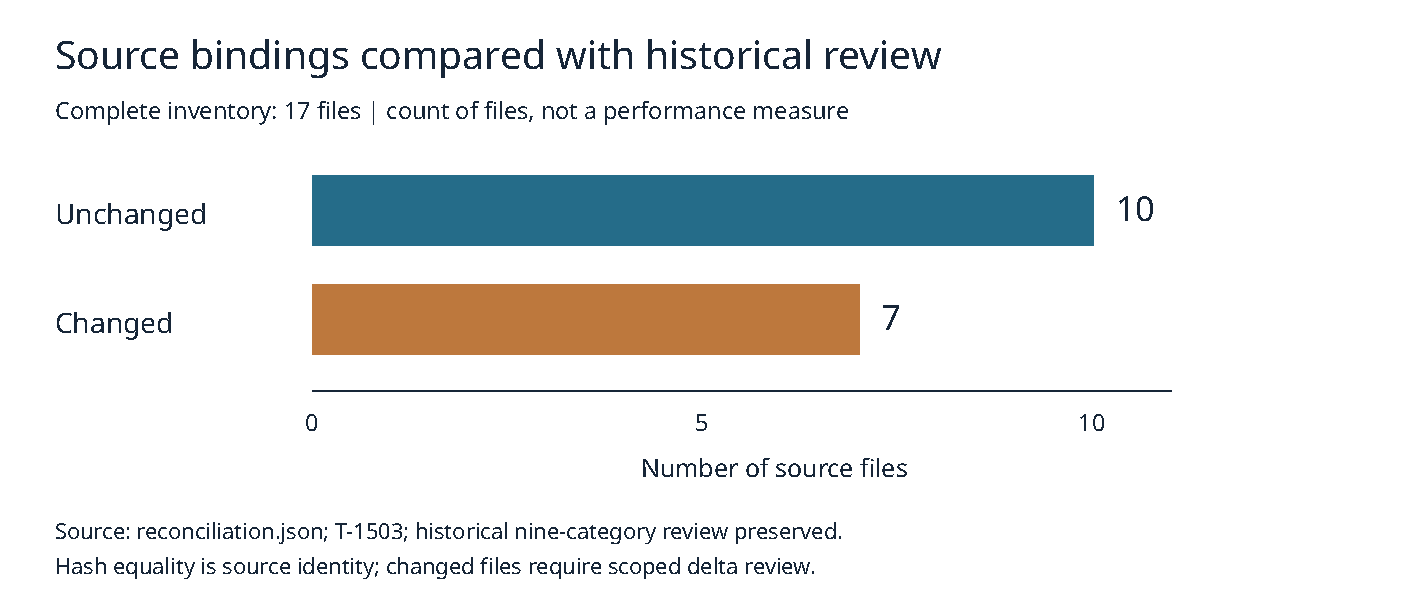
\includegraphics[width=\linewidth]{source-bindings.pdf}\end{center}
\textbf{Evidence.} Source inventory: \texttt{../reconciliation.json}; all 17 rows and exact old/current SHA256 values are in \texttt{source-comparison.csv}. Original packet commit: \texttt{e866228027}. Historical review: \path{finite_coverage_run_binding_20261030/coverage-review.json}. Original binary begins \texttt{a1c8ca89}; protocol body begins \texttt{cf8f76ea}. The graph is a complete fixed inventory; no sampling interval is applicable.

\textbf{Inspected changes.} Mapper/importer permit null session identities for unexecuted plans, while actual records still require a concrete session. The inspected mapper change does not alter arithmetic pricing. Rho event changes are test-only; the library exports a reporting module. Native solver and pencil adapters add trace/progress routes and move applicability checks. Actual selected routes and added dependencies require source-specific review.
\newpage
\section*{Historical scope and precise next bindings}
The nine historical categories are: field arithmetic; scalar arithmetic; outer and constructor validation; setup and transfer; collection, graph and elimination; hash and RNG; source verification; metadata clone; calibration. Each is marked covered in the preserved historical review. Ten unchanged hashes permit exact reuse where the later review justifies it; seven changed hashes are not a blanket rejection of the model.

\textbf{Existing mapping.} Atomic inverse normalization already removes expanded multiplications. Cold setup, geometry segments and calibration have explicit disjoint treatment. The finite grid contains 36 declared algorithm-price cells; none are evaluated here. Diagnostic aggregate counters are excluded to prevent double counting.

\textbf{Candidate obligations.} Bind the final finite-difference recurrence source, its initialization/update arithmetic and collection primitives, actual route, producer/reference binaries, mapper and prospective protocol. Check exact sieve output equality and phase/counter correspondence before review. Rebind all nine source categories, preserving prior coverage where source and semantics agree. Retain failed/capped/missing pairs as null outcomes and aggregate prescribed matched sums.

\textbf{Separate resources.} Allocation, JSON/serialization/digest work, observer traversal, process/harness costs, wall/CPU/RSS and infrastructure/retries retain their own units. They have no invented GAE coefficient. This finite model is not an all-instruction or total-dollar census.

\textbf{Cohort decision.} Preserve historical p739 records as old-arm evidence. Output equivalence does not convert old operation counts into optimized-candidate prices. The coordinator requires new candidate execution across all 1,260 original targets, under the remaining prospective execution gates.

\textbf{Provenance and limitations.} This is an additive source reconciliation by an agent with integration context, not a blind independent review. Historical records remain unchanged. No pricing calculation, test, scientific execution or runtime launch was performed. Sources inspected include the current native-price analyzer/importer/README, meter, scalar ledger, native solver, cost draft and retained historical finite source review. Exact source comparisons are retained in the JSON and CSV for independent inspection.
\end{document}
